\subsection{بخش ح}
در این بخش بر اساس شرایط اولیه داده شده،  قانون هدایت فرمان به خط دید با جبران‌سازی شتاب گرانش با قانون هدایت خط دید پایه مقایسه شده است.

\begin{table}[H]
	\caption{فاصله ازدست‌دهی در قانون هدایت فرمان به خط دید و جبران‌سازی شتاب گرانش با قانون هدایت خط دید پایه}
	\centering
	\begin{tabular}{cc}
		\hline
		\lr{Miss Distance (m)} & \lr{Guidance Law} \\
		\hline
		\lr{5.1732}  &\lr{BLOS}   \\
		\lr{4.8192 }&\lr{CLOS}   \\
		\hline
	\end{tabular}
\end{table}

\begin{figure}[H]
	\centering
	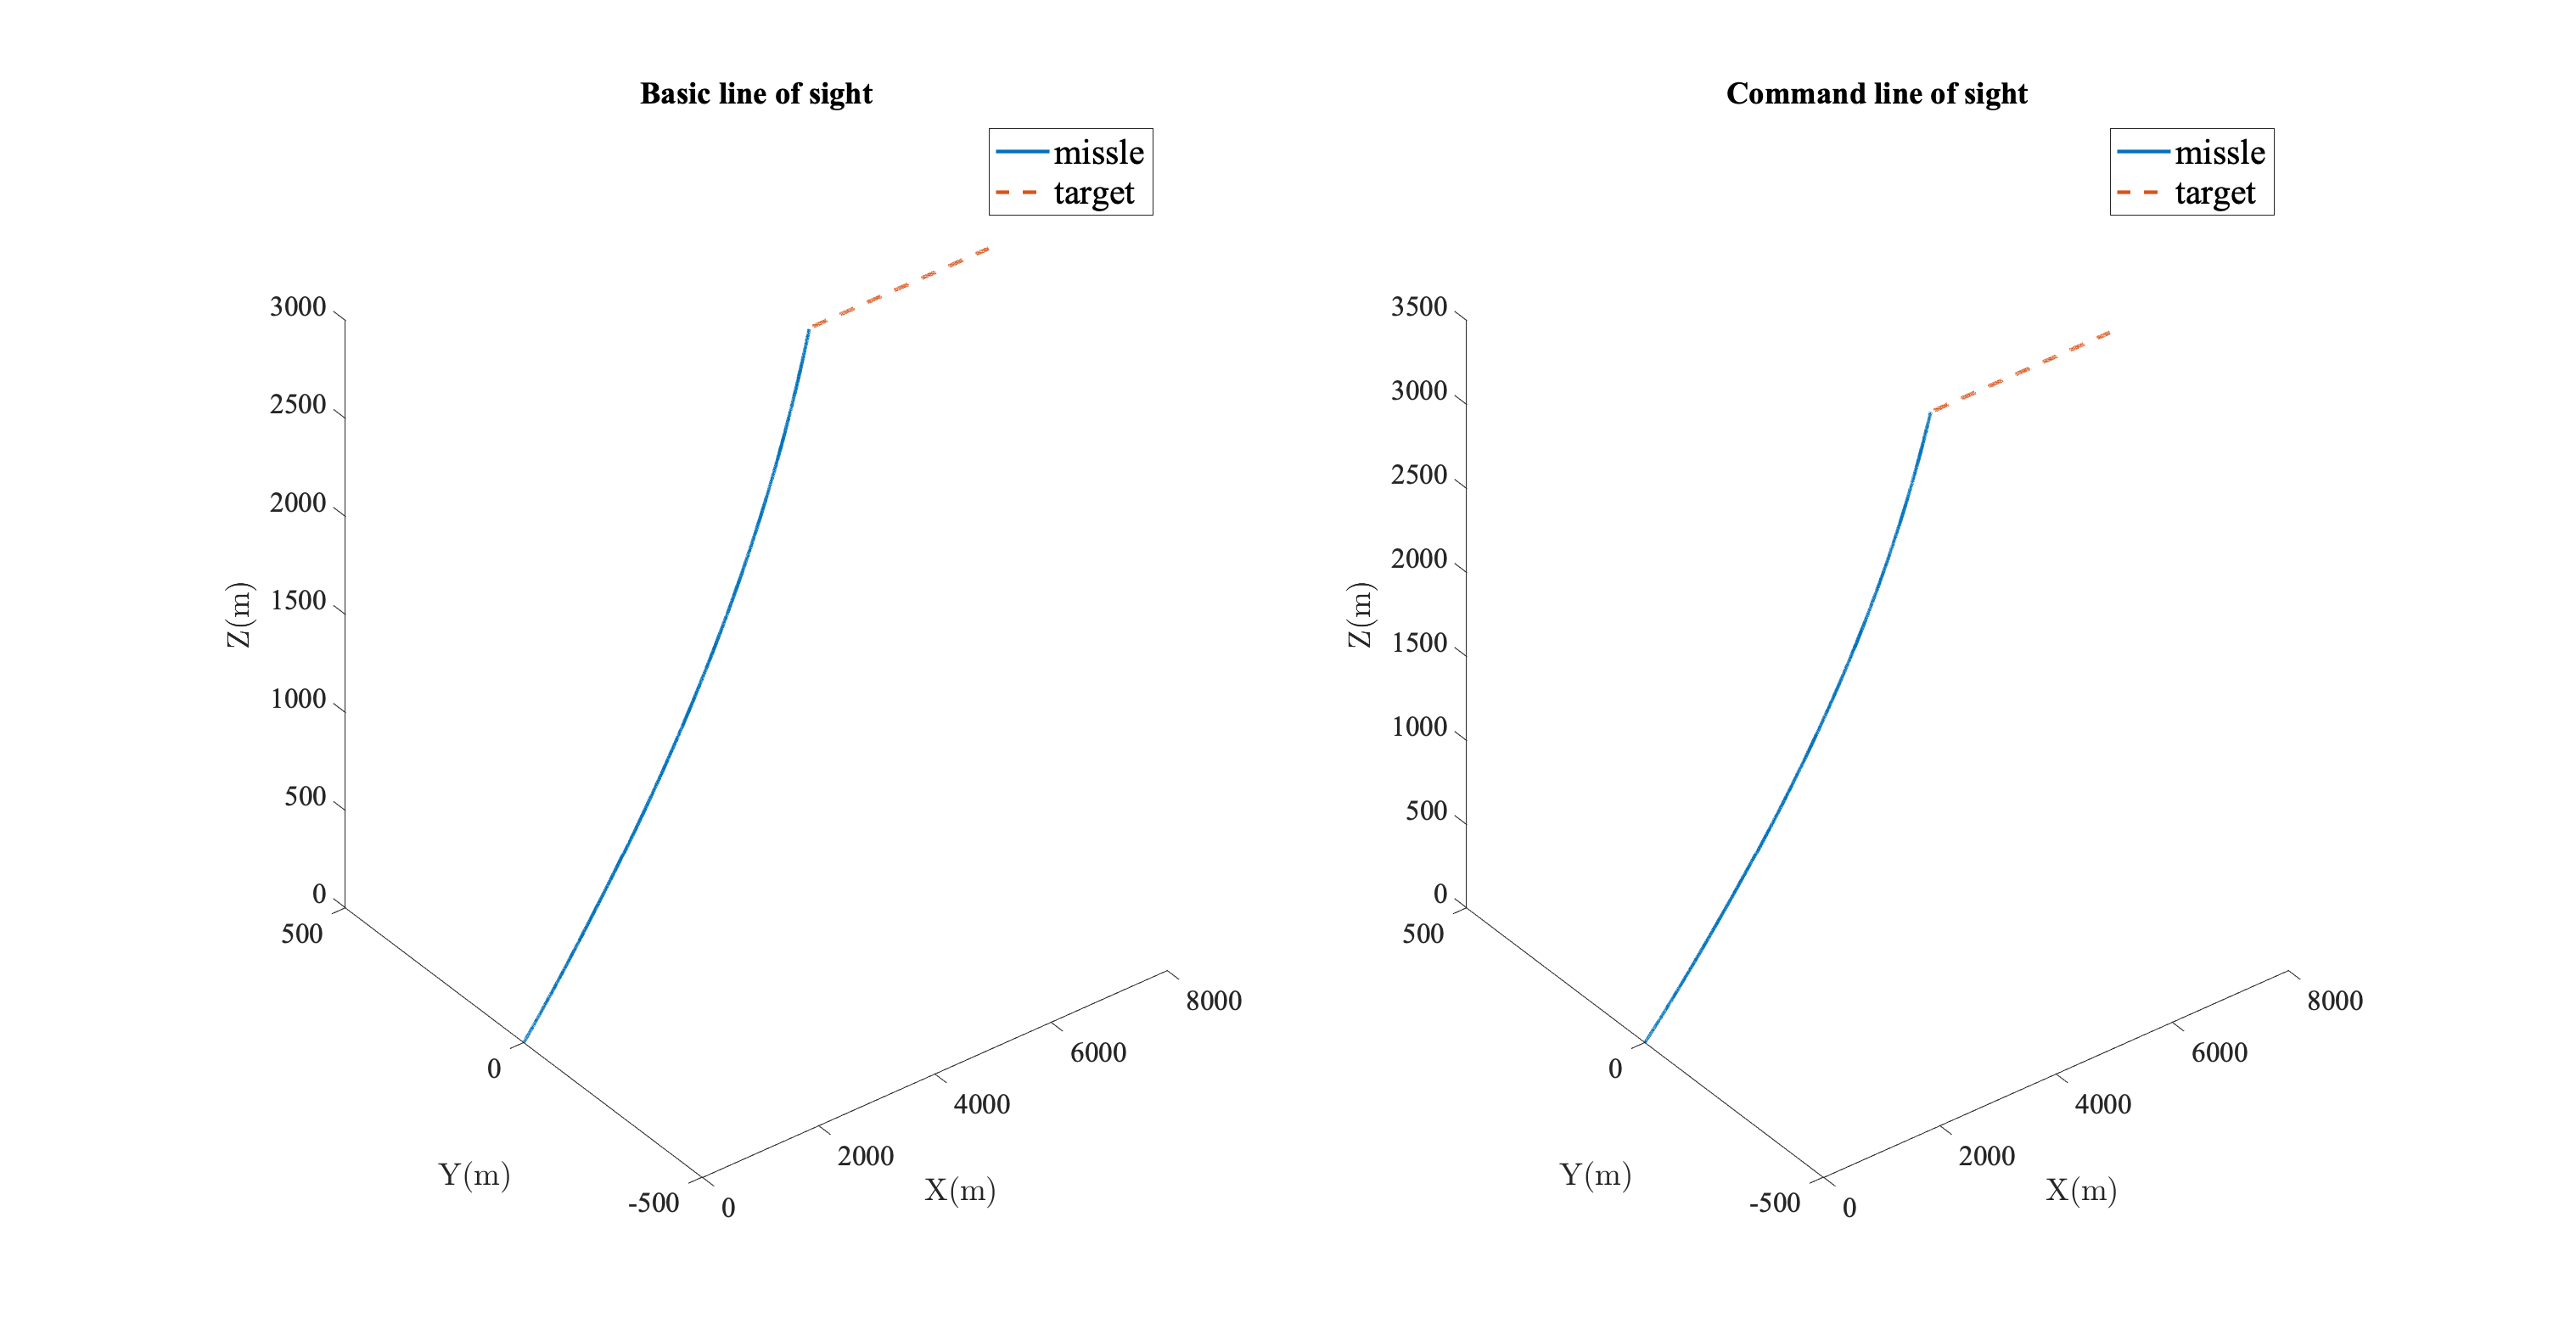
\includegraphics[width=\linewidth]{../Figure/h/3DoF_missle_vs_target_state}
	\caption{مقایسه موقعیت موشک و هدف به صورت سه بعدی در دو نمودار در قانون هدایت فرمان به خط دید و جبران‌سازی شتاب گرانش با قانون هدایت خط دید پایه }
\end{figure}

\begin{figure}[H]
	\centering
	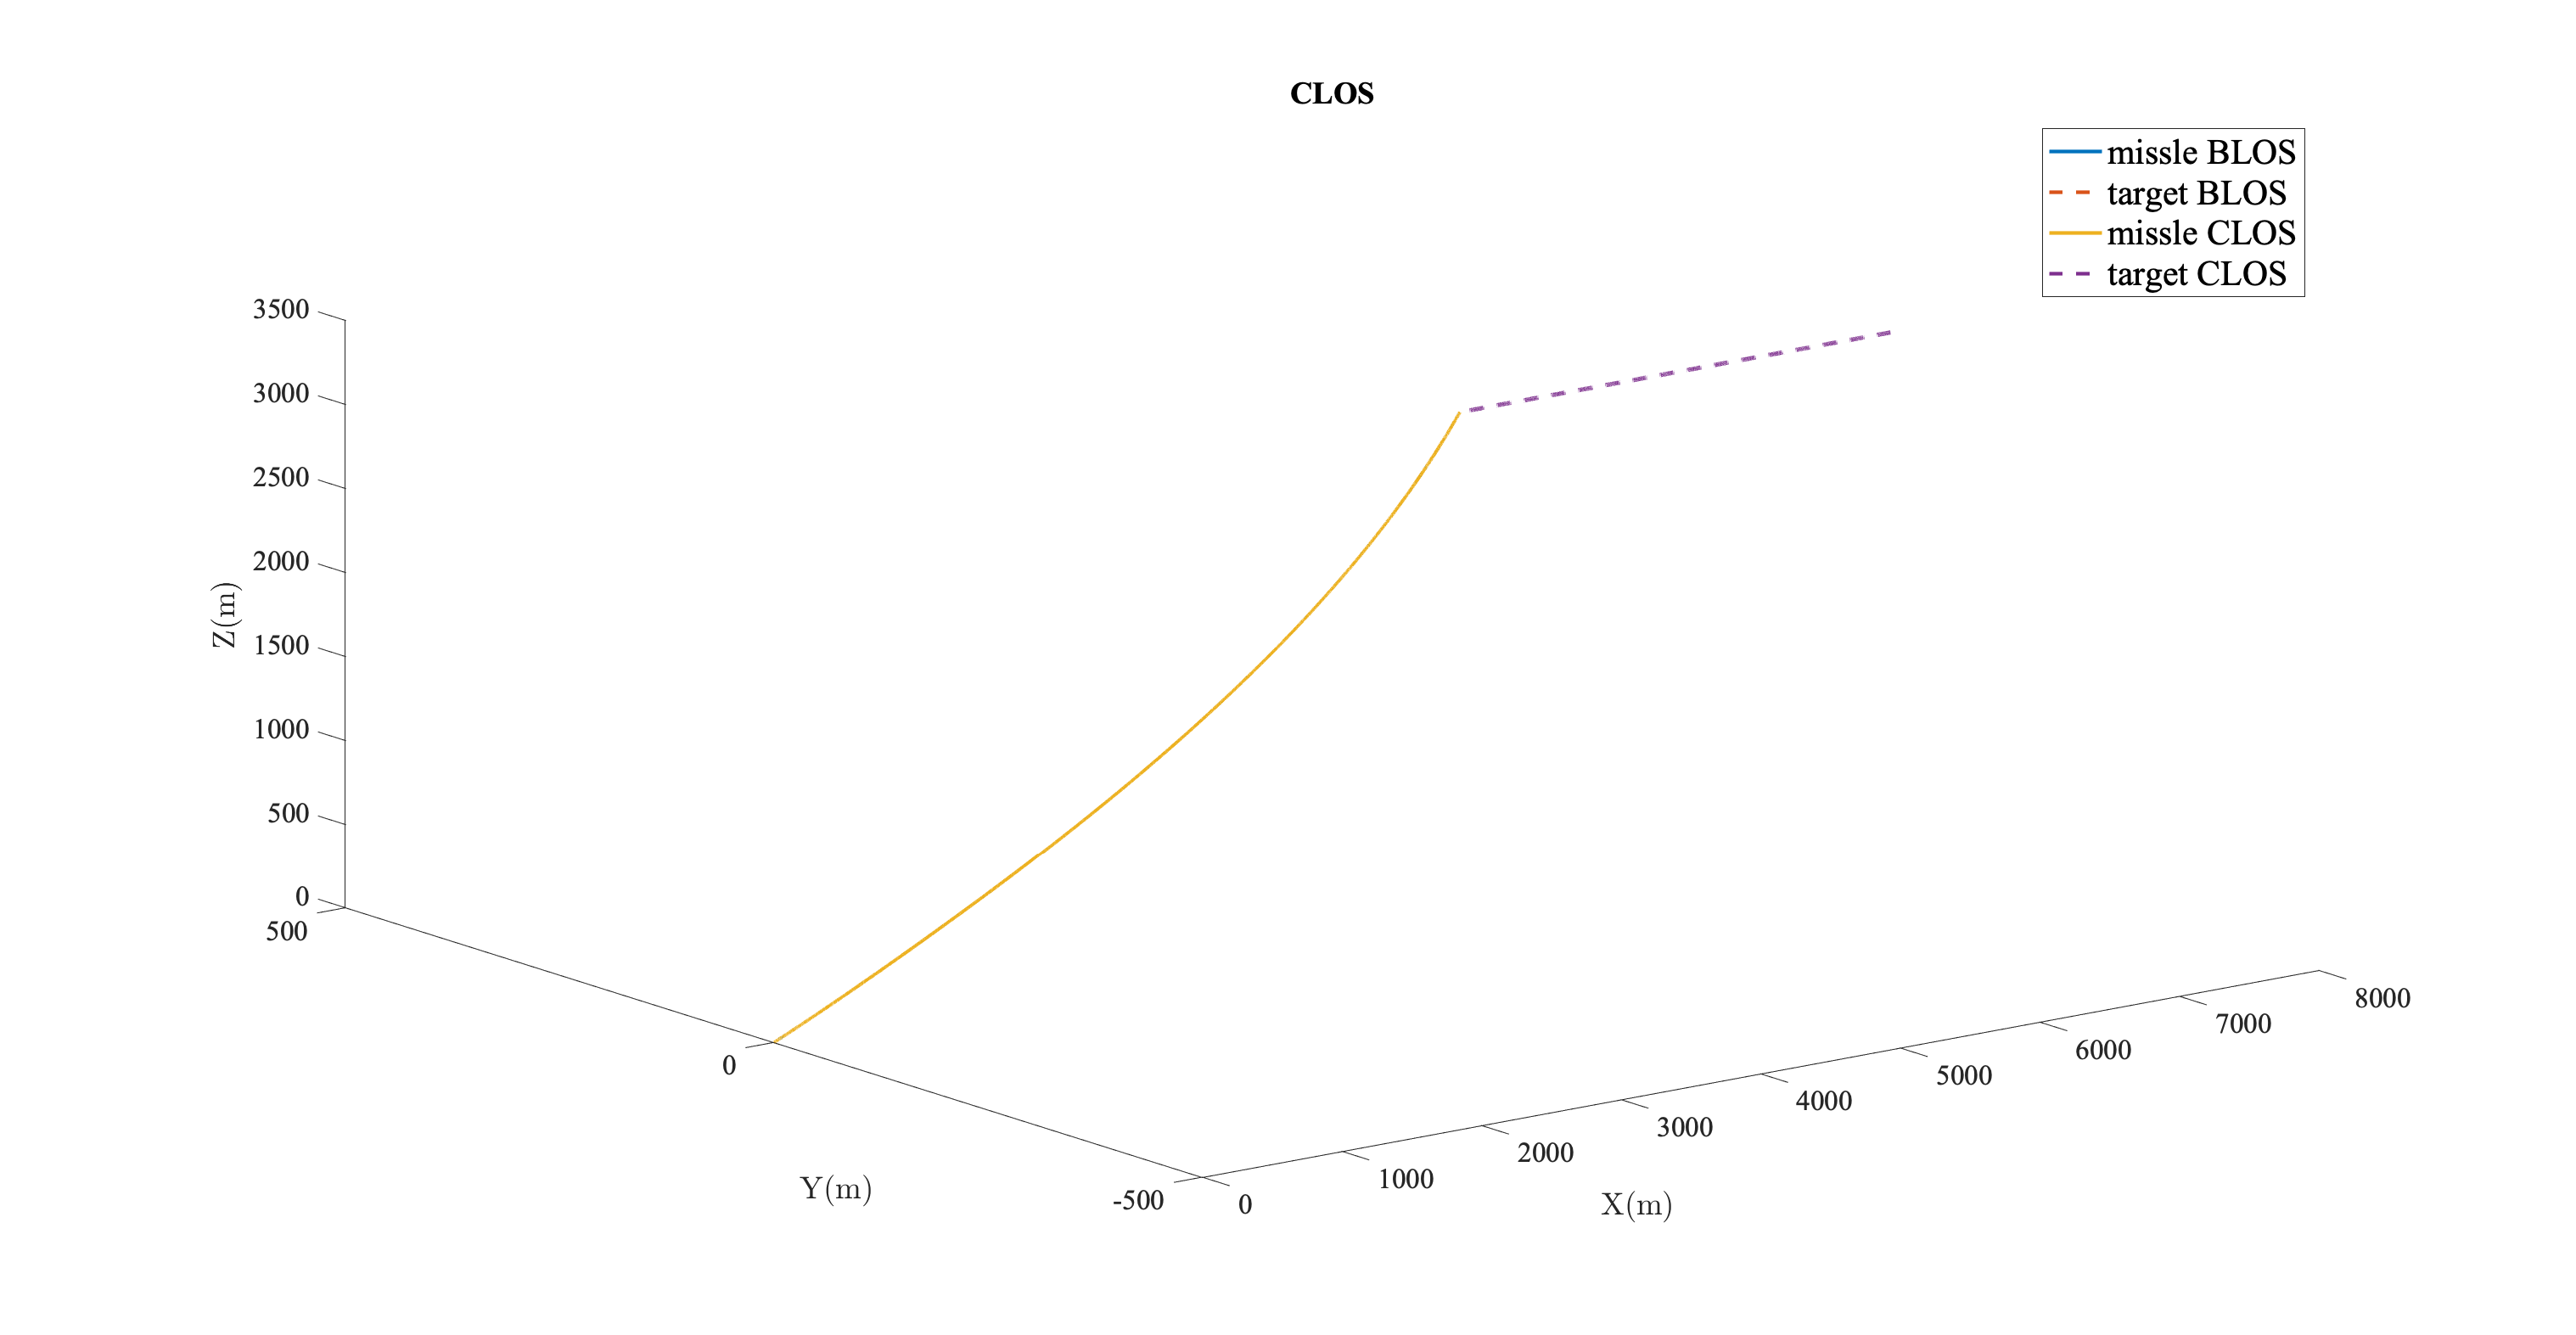
\includegraphics[width=\linewidth]{../Figure/h/3DoF_missle_vs_target_state_all_in}
	\caption{مقایسه موقعیت موشک و هدف به صورت سه بعدی در یک نمودار در قانون هدایت فرمان به خط دید و جبران‌سازی شتاب گرانش با قانون هدایت خط دید پایه }
\end{figure}

\begin{figure}[H]
	\centering
	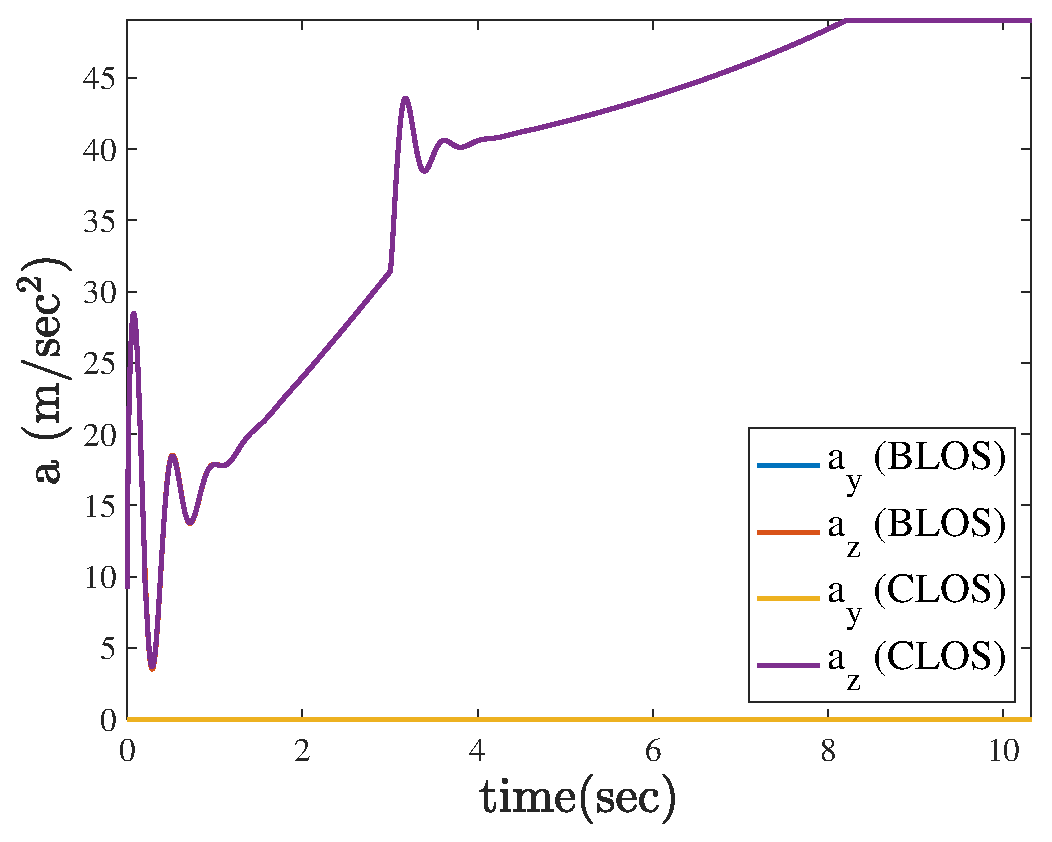
\includegraphics[width=.75\linewidth]{../Figure/h/command}
	\caption{مقایسه فرمان موشک در قانون هدایت فرمان به خط دید و جبران‌سازی شتاب گرانش با قانون هدایت خط دید پایه }
\end{figure}

\begin{figure}[H]
	\centering
	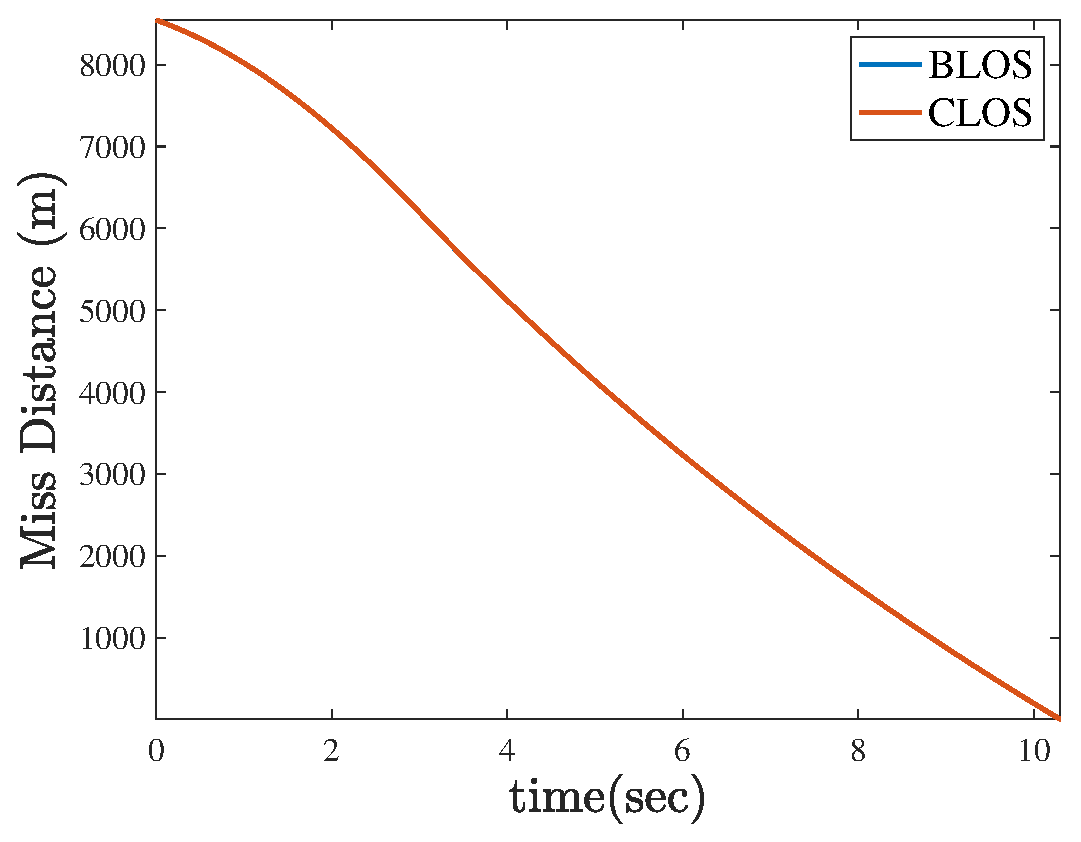
\includegraphics[width=.75\linewidth]{../Figure/h/miss_distance}
	\caption{مقایسه فاصله ازدست‌دهی موشک در قانون هدایت فرمان به خط دید و جبران‌سازی شتاب گرانش با قانون هدایت خط دید پایه }
\end{figure}
